%%\documentclass[onecolumn, draftclsnofoot,10pt, compsoc]{IEEEtran}
\documentclass[journal,10pt,onecolumn,compsoc]{IEEEtran} 
\usepackage[margin=1.0in]{geometry} 
%%\geometry{textheight=9.5in, textwidth=7in}
\usepackage{pdfpages}
%\usepackage{graphicx}
\usepackage{caption,graphicx,float} 
\usepackage{listings}
\usepackage{verbatim}
\usepackage[english]{babel}
\usepackage{url}
\usepackage{setspace}
%\setlength{\parskip}{\baselineskip} 
\setlength\parindent{24pt}

% 1. Fill in these details
\def \CapstoneTeamName{			HART CS Capstone}
\def \CapstoneTeamNumber{		11}
\def \GroupMemberOne{			Rick Menzel}
\def \GroupMemberTwo{			Matthew Forsland}
\def \CapstoneProjectName{		High Altitude Rocketry Project}
\def \CapstoneSponsorCompany{		OSU American Institute of Aeronautics and Astronautics (AIAA)}
\def \CapstoneSponsorPerson{		Dr. Nancy Squires}

% 2. Uncomment the appropriate line below so that the document type works
\def \DocType{			%Problem Statement
				%Requirements Document
				%Technology Review
				Design Document
				%Progress Report
				}
			
\newcommand{\NameSigPair}[1]{\par
\makebox[2.75in][r]{#1} \hfil 	\makebox[3.25in]{\makebox[2.25in]{\hrulefill} \hfill		\makebox[.75in]{\hrulefill}}
\par\vspace{-12pt} \textit{\tiny\noindent
\makebox[2.75in]{} \hfil		\makebox[3.25in]{\makebox[2.25in][r]{Signature} \hfill	\makebox[.75in][r]{Date}}}}
% 3. If the document is not to be signed, uncomment the RENEWcommand below
%\renewcommand{\NameSigPair}[1]{#1}

%%%%%%%%%%%%%%%%%%%%%%%%%%%%%%%%%%%%%%%
\begin{document}
\begin{titlepage}
    \pagenumbering{gobble}
    \begin{singlespace}
    	
\includegraphics[height=4cm]{coe_v_spot1}
        \hfill 
        % 4. If you have a logo, use this includegraphics command to put it on the coversheet.
        %\includegraphics[height=4cm]{CompanyLogo}   
        \par\vspace{.2in}
        \centering
        \scshape{
            \huge CS Capstone \DocType \par
            {\large\today}\par
            \vspace{.5in}
            \textbf{\Huge\CapstoneProjectName}\par
            \vfill
            {\large Prepared for}\par
            \Huge \CapstoneSponsorCompany\par
            \vspace{5pt}
            {\Large\NameSigPair{\CapstoneSponsorPerson}\par}
            {\large Prepared by }\par
            Group\CapstoneTeamNumber\par
            % 5. comment out the line below this one if you do not wish to name your team
            \CapstoneTeamName\par 
            \vspace{5pt}
            {\Large
                \NameSigPair{\GroupMemberOne}\par
                \NameSigPair{\GroupMemberTwo}\par
            }
            \vspace{20pt}
        }
        \begin{abstract}
        % 6. Fill in your abstract
		This document is intended to outline the design and system architecture for the OSU High Altitude Rocketry team's Avionics Ground System.
		It begins with a system overview, followed by a discussion of the design viewpoints which influenced the system.
		It then details the functionality of the final system as well as the design decisions made in the interest of providing this functionality, including a breakdown and explanation of each system component.
        	%This allows you to have sensible diffs when you use \LaTeX with version control, as well as giving a quick visual test to see if sentences are too short/long.
        	%If you have questions, ``The Not So Short Guide to LaTeX'' is a great resource (\url{https://tobi.oetiker.ch/lshort/lshort.pdf})
        \end{abstract}     
    \end{singlespace}
\end{titlepage}
\newpage
\pagenumbering{arabic}
\tableofcontents
% 7. uncomment this (if applicable). Consider adding a page break.
%\listoffigures
%\listoftables
\clearpage


\setlength{\parskip}{\baselineskip} 
% 8. now you write!
\section{Table of Changes}

\begin{center}
\begin{table}[h!]
\begin{tabular}{|p{0.3\linewidth}|p{0.3\linewidth}|p{0.3\linewidth}|} 
	\hline
	\textbf{Section} & \textbf{Original} & \textbf{New} \\
	\hline
	6 (Figure 2) & Originally had an image of a draft design. & Updated with final gauge design image. \\ 
	\hline
	6.1 & Originally intended to have separate vertical and horizontal acceleration gauges with positive and negative regions. Normal zones were originally going to be green. & Combined acceleration into a single gauge for each rocket stage due to space constraints and because the total force is the important aspect. Gauge now shows absolute value due the aforementioned reason and due to data format from instrumentation. Opted not to color normal zone on gauge.\\
	\hline
  6.2 & Was originally altitude. & Moved to 6.4. 6.2 now discusses the Temperature gauge.\\
  \hline
  6.2.1 & Discussion of audible cues was somewhat vague. & Specified that audible cues are a flex goal. \\
  \hline
	6.3 & Was originally barometric pressure. & Scrapped that component following user testing. 6.3 Is now Velocity. Originally intended to have a gauge with positive and negative regions. Normal zones were originally going to be green. Velocity gauge now shows absolute value due the the total force being the important aspect and due to data format from instrumentation. Opted not to color normal zone on gauge.\\
	\hline
  6.4 & Was originally thrust gauge. & Scrapped that component due to lack of access to scripts we had previously been told the client would provide. 6.4 is now Altitude. Added image of readouts above 6.4.\\
  \hline
  6.5 & Was the Velocity Gauge. & Moved to 6.3. 6.5 is now GPS coordinates. \\
	\hline
  6.6 & Originally had no image. & Added image of Position display. \\
  \hline
  7.2 & Was blank. & Added image of final desktop dashboard. \\
  \hline
  7.3 & Was blank. & Added discussion of layout and user interactivity.\\
  \hline
\end{tabular}
\caption{Table of Changes}
\label{table:1}
\end{table}
\end{center}
\newpage

\section{Introduction}

	\subsection{Scope}
		\noindent The Avionics Ground System described herein is intended to provide ground-level near real-time location and status information during launches of the OSU AIAA High Altitude Rocketry Team's rocket.
		The goal of providing this information is two-fold: firstly, to facilitate timely recovery of both rocket stages post-flight; secondly, to allow the ground team to monitor the flight, most notably the altitude.

	\subsection{Purpose}
		\noindent This Design Document serves as an overview of how the final Avionics Ground System shall be designed and implemented.
		To this end, this document will outline the various requirements of the final system, as well as detail the specific design and architecture designs made to fulfill these requirements.

	\subsection{Intended Audience}
		\noindent This document is intended for the several technical stakeholders in the 2018-2019 OSU AIAA High Altitude Rocketry team.
		It is to be used as a road-map for the HART CS capstone team (hereafter referred to as the "development team") during the coming implementation of the ultimate system.
		Finally, the Design Document is intended to serve as the document-of-reference for all stakeholders in the event of later conflict between the final system and its stated requirements.

	\subsection{Conformance}
		\noindent As written, this document conforms to the requirements and specifications requested by the project client and later enumerated by the development team as of November 24th, 2018.
		As of the time of this writing, both client and development team have agreed upon the scope of the intended system.
		Records to this effect are maintained by the development team.
		Further information regarding the agreed upon project requirements and specifications may be located in the Requirements Document.

	\subsection{Reference Material}
		\noindent [1]"COCOM - COCOM GPS Tracking Limits | Coordinating Committee for Multilateral Export Controls", Ravtrack, English, 2018. [Online]. Available:http://ravtrack.com/GPStracking/cocom-gps-tracking-limits/469/. [Accessed: 25- Nov- 2018].
		
		\noindent [2]"Avionics Definition", Merriam-Webster, English, 2018. [Online]. Available:https://www.merriam-webster.com
		\noindent /dictionary/avionics. [Accessed: 25- Nov- 2018].
		
		\noindent [3]"About AIAA", AIAA, English, 2018. [Online]. Available:https://www.aiaa.org/AboutAIAA/. [Accessed: 25- Nov- 2018].

	\subsection{Definitions and Acronyms}
	\begin{itemize}
		\item \textbf{AIAA:}
			American Institute of Aeronautics and Astronautics. \\
		
		\item \textbf{Avionics:}
			electronics designed for use in aerospace vehicles. \\
		
		\item \textbf{Back-End:}
			The non-user-facing components of the Avionics Ground System. \\
		
		\item \textbf{COCOM:}
			An abbreviation for "Coordinating Committee for Multilateral Export Controls."
			It ceased to function in 1994, but has a legacy of GPS restrictions preventing GPS-guided ballistic missiles.
			These restrictions will affect the telemetry available for a period of the rocket's flight when it exceeds 515 meters per second and 18 kilometers altitude above ground level. \\
		
		\item \textbf{GPS:}
			Global Positioning System. \\
		
		\item \textbf{Ground Station:}
			The ground based receiver and broadcast system used by HART. 
			Based on a Raspberry Pi, the ground station receives telemetry from the rocket, processes it, and then broadcasts it over Wi-Fi for view. \\
		
		\item \textbf{GUI:}
			Graphical User Interface. \\
		
		\item \textbf{ECE:}
			Electrical and Computer Engineering \\
		
		\item \textbf{Front-End:}
			The user-facing components of the Avionics Ground System. \\
		
		\item \textbf{HART:}
			High-Altitude Rocketry Team \\
		
		\item \textbf{ME:}
			Mechanical Engineering	\\
		
		\item \textbf{OSU:}
			Oregon State University \\
		
		\item \textbf{USC:}
			University of Southern California \\
	
	\end{itemize}

\newpage

%-----------------------------------------------------------

\section{System Overview}
	%\noindent The OSU chapter of the AIAA is seeking to break the current collegiate high-altitude record for a student-built rocket.
	%The current altitude record, set by a team from USC, is 144,000 feet.
	%This effort will build on projects from previous years (2016-2017, 2017-2018) and is part of a long-term effort to win the University Space Race, a challenge to launch a student-built rocket to an altitude of 100 kilometers.
	%To this end, HART will design and assemble a 2-stage solid-rocket motor, to be launched June 2019 at the Spaceport America Cup in New Mexico. 

	%\noindent Amateur high-powered rockets flying in excess of 5000 feet are no longer visible to the naked human eye. 
	%Depending on the weather, time of day, and location of the launch pad relative to the observer, the rocket may potentially be obscured by the sun or cloud cover, further complicating visual tracking efforts. 
	%As such, HART's rocket must broadcast telemetry containing, at a minimum, some measure of altitude and position.
	%This telemetry must then be received, interpreted and finally displayed to personnel on the ground.
	%Because HART is a multi-disciplinary effort, the overall avionics system is divided among two sub-teams.
	%ECE and ME sub-teams have responsibility for the broadcast of telemetry data, as well as the avionics hardware which will be integrated into the rocket.
	%Together these components make up the Avionics Flight System.
	%The CS sub-team is then responsible for receiving this telemetry, processing the data into a usable form, and displaying relevant information in an easily digestible manner.
	%To achieve this functionality, the CS portion of the system, the Avionics Ground System, will be further divided into a back-end and a front-end.
  
	%some stuff about the back-end

	%\noindent Once received data is processed by the front-end, it is passed to the front-end.
	%The front-end has two broad functions.
	%Firstly, it is the front-end which is responsible to displaying the position of both rocket stages during and immediately following flight.
	%This includes both near real-time positions and a persistent flight path derived from positions previously reported.
	%This location display is primarily intended as an aid to the ultimate recovery of the rocket stages post-flight, but also serves the ancillary goal of monitoring for any emergent in-flight conditions which effect the flight path of the rocket.
	%Secondly, the front-end is responsible for displaying a full range of received and derived telemetry data to users.
	%This data includes the rocket’s altitude, vertical and horizontal velocity, acceleration, barometric pressure and the thrust achieved from the rocket motors.
	%Both of these functions will be implemented via a web-based interface hosted off of the ground station and accessible to any team member with a web-enabled device via connection to the ground station's integrated router. 

	% Problem statement
	\noindent Amateur high-powered rockets flying in excess of 5000 feet are no longer visible to the naked human eye. 
	Depending on the weather, time of day, and location of the launch pad relative to the observer, the rocket may potentially be obscured by the sun or cloud cover, further complicating visual tracking efforts. 
	As such, HART's rocket must broadcast telemetry containing, at a minimum, some measure of altitude and position.
	This telemetry must then be received, interpreted and finally displayed by the ground station system to personnel on the ground.
	Because HART is a multi-disciplinary effort, the avionics and ground station systems are divided among two sub-teams.
	The ECE sub-team is responsible for the broadcast of telemetry data, as well as the design and manufacture of the avionics hardware which will be integrated into the rocket.
	The CS sub-team is responsible for receiving this telemetry, processing the data into a usable form, and displaying relevant information in an easily digestible manner.
	To achieve this functionality, the CS portion of the ground station system will be further divided into a back-end and a front-end.
	
	% Backend overview
	\noindent The back-end subsystem will receive raw telemetry data from the rocket via an omni-directional radio antenna.
	Received telemetry will contain measurements of temperature, barometric altitude, accelerometer, gyroscopic orientation, and GPS position when available.
	These measurements will be used to update an internal model of the positions of both rocket stages.
	The internal model will reduce noise in the telemetry data and allow for interpolation of rocket velocity and thrust achieved by the rocket motors.
	Raw telemetry data and processed data from the model will be output to files for long-term storage, further analysis, and use by future HART teams.
	
	%Frontend overview
	\noindent Once data is processed by the back-end, it is passed to the front-end.
	The front-end has two broad functions.
	Firstly, it is the front-end which is responsible for displaying the position of both rocket stages during and immediately following flight.
	This includes both near real-time positions and a persistent flight path derived from previously reported positions.
	This location display is primarily intended as an aid to the ultimate recovery of the rocket stages post-flight, but also serves the ancillary goal of monitoring for any emergent in-flight conditions which affect the flight path of the rocket.
	Secondly, the front-end is responsible for displaying a full range of received and derived telemetry data to users.
	This data includes the rocket’s altitude, vertical and horizontal velocity, acceleration, barometric pressure and the thrust achieved from the rocket motors.
	Both of these functions will be implemented via a web-based interface hosted off of the ground station and accessible to any team member with a web-enabled device via connection to the ground station's integrated router. 

	
%-----------------------------------------------------------

\section{System Architecture}
	\noindent This section provides a conceptual model for the ultimate Avionics Ground System, and describes in detail the various components alongside their respective implementations.
	It first establishes the Architectural Design by defining the relationship of each component with respect the the overall system.
	After this, the Decomposition Description breaks down and describes the actual features intended to be present in the final solution.
	Finally, the Design Rationale sub-section elucidates the general reasoning which influenced the above-described design.

	\subsection{Architectural Design}

		\begin{figure}[H]
		\fbox{\includegraphics[width=\textwidth]{flow.eps}}
		\caption{Basic Data Architecture}
		\end{figure}

		\noindent The application shall consist of a single web page (hereafter referred to as the "main page") which will allow users to monitor telemetry and location for both rocket stages in near real-time both during and immediately proceeding flight.
		This page will feature two sections.
		The first section is responsible for displaying the current location(s) and flight path of the rocket 3-dimensionally.
		Users will be able to manipulate the 3-dimensional portion of the display to change the viewing angle.
		The second section is responsible for displaying other telemetry including the rocket’s altitude, vertical and horizontal velocity, acceleration, barometric pressure and thrust.
		This will be accomplished via a series of 2-dimensional gauges and numerical readouts as is most appropriate to the specific parameter being displayed.
		Data will be displayed both during and immediately following flight.

		\noindent The back-end shall consist of a system responsible for receiving the telemetry of both stages, two systems for modeling the state of each rocket stage, and one system responsible for passing processed data to the front-end.
		The data reception system will receive raw telemetry data directly from the antenna and parse it into the different variables contained within.
		Once parsed, the system will store those variables to a file, and write them to a pipe connected to the data processing systems.
		The data processing subsystems will derive velocity from the incoming data, and use it together with the raw data to update an internal model designed to remove experimental noise.
		The data processing subsystem will also use the model to estimate the thrust produced by the motor between each transmission.
		The outputs of the model and the thrust will also be written to a file, and to a pipe connected to the data delivery system.
		The data delivery system will retrieve live data from the data processing system during flight, or read old flight data from a file, and send it to the front-end.
		
	\subsection{Decomposition Description}
		\noindent Data will flow into the data reception subsystem from the antenna receiving telemetry transmissions from the rocket stages.
		The raw telemetry will be stored to a file and sent to the data processing subsystem.
		The data processing subsystem will refine the raw telemetry into single measurements, eliminate experimental noise, and derive additional variables not directly measured.
		The data processing subsystem will store all refined and derived variables to a log file, and send them to the data delivery system.
		The data delivery subsystem will send refined data from a live flight to the front-end by receiving data from the data processing subsystem.
		The data delivery subsystem will send refined data from a previous flight to the front-end by reading it from a file.

	\subsection{Design Rationale}
		\noindent The primary influence on the design of the Avionics Ground System is to present all information in a format which is easily and rapidly digestible.
		This should allow users to quickly glance at the page and within seconds get a basic grasp on the status of the rocket.
		Much of this rapid-assessment functionality will be provided by color-coding.
		Importantly, for much of the telemetry data it is not as important that values remain constant as it is that they remain within a nominal range. 
		By color-coding nominal value ranges to green, warning ranges to yellow, and danger ranges to red it should only take seconds for a user to determine whether the rocket is performing as expected or whether there is cause for concern.
		Similarly, the use of appropriate colors for the location and trajectory display will allow for a more rapid assessment.
		In both of these cases, a user will be able, if needed, to obtain more detailed information by conducting a closer examination of the readout, should such detail become necessary.

		\noindent In the course of a flight, the rocket stages will rotate rapidly, vibrate, and shake violently as the fins  spin-stabilize the rocket, the motors create acoustic vibrations that propagate through the entire rocket, and the stages fall under parachute.
		Furthermore, some measurements become unreliable when certain conditions are met, such as the barometer reading a spike in pressure as a shockwave forms around the rocket when it passes Mach 1.
		All of these tendencies and events will generate a significant amount of experimental noise in the raw telemetry.
		In order to present more digestible data, it is imperative that an algorithm be used to reduce this noise.
		As such, the data processing subsystem will employ a Kalman filter to model the rocket stages' statuses and mitigate experimental noise according to statistical analysis.
		
\newpage

%-----------------------------------------------------------

\section{Avionics Ground System Perspective}
	\subsection{Design Stakeholders and Concerns}
		\noindent From the perspective of the development team, it is desirable to produce a system which is modular in nature.
		With the key considerations that other portions of both the overall Avionics System and the airframe are subject to change throughout our development timeline, this modularity will lend itself to the flexibility and maintainability of the system.
		Furthermore, a modular system has the potential to allow for the addition of optional features should time allow.
		Lastly, it is critical that the system be designed with the constraints of the available hardware foremost in the mind, both in terms of processing power (which is limited) and supported APIs (also likely limited).
		
		\noindent The development team, is however, only a small part of HART.
		Because of the diverse makeup of the rest of the team and the highly time sensitive nature of the final launch attempt, it is important for the final system to be simple to operate and understand.
		This element of understanding is further significant due to the amount of information being communicated: the final design should be one which lends itself to easy and rapid assessment.

	\subsection{Design Viewpoints}
		\noindent This section describes several different viewpoints regarding the HART Avionics Ground System, namely context, interface, structure and interaction.

		\subsubsection{Context Viewpoint}
			\noindent A critical concern in the development of the overall avionics system is the varying disciplines of the intended users. 
			Specifically, HART is a multidisciplinary team composed primarily of Mechanical Engineering students (and one Mechanical Engineering faculty member) with several supplemental sub-teams made up of Electrical and Computer Engineering students, a Chemical Engineering student, and two Computer Science students (the CS sub-team).
			As such, the level of familiarity with software and programming can be expected to differ substantially between team stakeholders.
			This consideration drives a need to produce software which is inherently simple to access, run and navigate, so as to avoid confusion or delay around the critical launch window. 

		\subsubsection{Interface Viewpoint}
			\noindent A key motivator for this project is to broaden the user interface beyond the ground station hardware.
			As such, a web-based design for the visualization system has been chosen, as this will allow multiple team members to access telemetry data from personal devices such as laptops or cellphones rather than requiring them to crowd around a single screen.
			This decision was further informed by the ground station hardware itself.
			As the ground station is powered by a Raspberry Pi (with no GPU), there is a distinct possibility that many graphical applications would be difficult or impossible to run on that system.
			Web-based approaches to visualization are, however, implemented directly by web browsers.
			This both ensures that the visualization will run and offloads the processing responsibility to the client's browser rather than the host machine.  

		\subsubsection{Structure Viewpoint}
			\noindent The multidisciplinary composition of HART further dictates a desire for a certain degree of modularity in the Avionics Ground System design.
			Specifically, the development team will need to begin software development prior to finalization of the Avionics Flight System (both software and hardware components) by the ECE and ME sub-teams.
			As such, it is entirely possible that some planned aspect of the broadcast system could change during the development of the display system.
			Modular design would minimize the impact of such changes by ensuring the number of effected components is kept to a minimum.
			Furthermore, modularity in the display system should allow for increased efficiency, in particular by offloading the graphical-processing responsibility to client machines and thus freeing the ground station to work more on processing and storing data. 

		\subsubsection{Interaction Viewpoint}
			\noindent A further offshoot of the above-discussed modularity is the desire for relatively independent system components.
			In other words, interaction between components should be kept to a minimum and performed only when necessary.
			This helps both to ensure an orderly flow of information through the program and potentially to avoid negative interactions in the event of system malfunction.
\newpage


%-----------------------------------------------------------

\section{Back-End Component Design}
	This section will explain the subsystems of the back-end ground station system.
	Each subsystem will be broken up into multiple components.
	Each component will be explained in two levels.
	These levels are Algorithm, Physical Implementation (only in the Telemetry sub-section), and Design Rationale.

	\subsection{Telemetry}
		\noindent This section will explain the design of the back-end subsystem responsible for the reception and storage of raw telemetry data from the rocket.
		
		\noindent Capturing accurate and reliable in-flight telemetry data is perhaps the most important problem in this project for several reasons. 
		Firstly, given that this effort is fundamentally a competition, both in terms of this year's attempt to best the current altitude record and the ultimate goal of winning the University Space Race, the ability to accurately monitor and record the altitude reached by our rocket is absolutely mission critical. 
		Secondly, after speaking to Dr. Squires, HART's faculty sponsor, it appears that last year's team was less than successful in capturing telemetry, a shortcoming which threatened the progress made by that team (as incomplete/inaccurate data is of questionable use). 
		As the ultimate goal of this project is to achieve a minimum altitude of 144,000 feet and the rocket is, of course, unmanned, capturing telemetry is the only way we will be able to determine success or failure.
		
		\noindent This section will additionally describe the physical hardware necessary for the component to function, where applicable.
		\setlength\parindent{0pt}
		\subsubsection{Data Reception}
		%\setlength\parindent{0pt}

			\paragraph{Algorithm}
				\noindent The telemetry data will be received via a socket from the external antenna.
				Once a packet is received, it will be decomposed into the various pieces of data contained within.
				When the rocket experiences specific events, such as stage separation, engine ignition, or parachute deployment, special packets will be broadcast signaling these events.
				When the rocket exceeds COCOM restrictions, GPS data will no longer be present in packets, and the structure of the packet will change accordingly.

				\noindent Once a packet has been decomposed into the set of data variables contained within, the variables will be reformatted into a JSON string and stored to a Flash drive.
				The variables will also be written to a pipe connecting the data reception subsystem to the data processing subsystem.
				The component must be fast enough that it is able to receive and store a packet of data faster than the rocket stages are able to transmit it.

			\paragraph{Physical Implementation}
				\noindent Telemetry data will be received by an omni-directional radio antenna designed and manufactured by the ECE sub-team.
				The antenna will connect to the ground station via USB cable, and will format the data as a packet addressed to the port the data reception subsystem is listening to on the ground station.

			\paragraph{Design Rationale}
				\noindent Stable reception of telemetry is vital to the accurate tracking of the rocketry stages.
				Using a directional antenna, while cheaper and easier to design, requires manually pointing the antenna at the suspected location of the rocket.
				Because the rocket will exceed the range within which it is visible to the human eye within the first seconds of flight, accurately tracking its position in such a manner is extremely unreliable.
				Using an omni-directional antenna requires a more powerful antenna overall, but does not require manual pointing, and needs to simply be held high enough to be clear to ground-based obstructions like shrubs, tents, and hills.
				Reformatting the incoming telemetry to be properly received by the listening port on the ground station will require some care when generating telemetry packets on the avionics system, but should not prove to be too much of an obstacle to the development of the telemetry transmission system.

		%\setlength\parindent{24pt}
		\subsubsection{Data Storage}
			\noindent Storing the received and processed telemetry data is not strictly necessary for the visualization system, but does allow for later analysis of the rocket's flight.
			This analysis could be performed by third-party software or by feeding the telemetry data back into the ground station system to simulate the live reception of the flight.
			This is important both to later demonstrate the flight's events, and to debug the rocket's systems based upon the emergence of unstable flight characteristics not predicted by the HART team.

			\noindent Given that this year's HART effort builds on work done in the two previous school years, the processing of data will be a significant first step. 
			There have been large amounts of unprocessed telemetry data collected from previous launches which offers a chance to analyze and subsequently improve upon earlier performance. 
			In particular, there is a significant amount of data on the in-flight thrust characteristics of these earlier rockets. 
			The processing and subsequent analysis of this data is central to HART's ability to improve upon OSU's existing launch capability not only in terms of altitude but also in reliability (which was an issue during last year's launch).

			\noindent Furthermore, the current HART team anticipates making several test launches prior to the ultimate competition launch at Spaceport America, including at least one full scale, full altitude test. 
			The ability to process and analyze data from these tests will allow us to improve the final airframe and thruster design as well as to detect and address potential issues along the way. 
			This ties into the second category: telemetry.


			\paragraph{Algorithm}
				\noindent Data will be written in a JSON format, which is easily parsed and clearly labeled, making it both human- and machine-readable.

			\paragraph{Physical Implementation}
				\noindent Data will be written to a file unique to the rocket stage and flight on a Flash drive.

			\paragraph{Design Rationale}
				\noindent The JSON format is easily parsed by computers, and most browsers automatically support the decomposition of a JSON object into a client-side memory construct to provide data for a web page.
				This will ease the transmission of data to the front-end system.
				Storing the data on an external Flash drive will make it much more accessible, as the Flash drive can be removed from the ground station and plugged into other, more powerful computers, to perform more specific analysis.

		\subsubsection{Telemetry Transmission to Data Processing Subsystem}
			\noindent Because the telemetry reception subsystem has the very tight time constraint of receiving transmissions in real time, it is safest to minimize the functional actions of the subsystem's process and interpret the telemetry on another process.
			Writing data to a separate function allows for a "fire and forget" approach, where data is written to a connecting bridge, and it is presumed that the other side is reading the data from the bridge at whatever pace is necessary.

			\paragraph{Algorithm}
				\noindent The received telemetry data will be written to a software pipe connected to the data processing subsystem.

			\paragraph{Physical Implementation}
				\noindent No physical hardware is necessary for a software pipe to function.

			\paragraph{Design Rationale}
				\noindent The telemetry could be moved between functions using ports and sockets, pipes, or files.
				All three methods give access to blocking read and write functions that force the receiving program to wait until a complete set of new data is written.
				Ports and sockets require significant configuration, but allow for the telemetry reception and processing systems to execute on separate computers.
				Because the ground station contains a single computer this is not necessary.
				Using a software pipe is slightly more efficient than using a temporary file to transmit data between the telemetry reception and processing systems

		\subsubsection{Telemetry Transmission to Front-end Subsystem}
			\noindent Similar to live reception of telemetry, sending telemetry to the front-end is time-critical to the live visualization of the flight.
			However, the code involved will be significantly different to the data processing system.
			It therefore makes more sense to extract it to a separate subsystem and reuse the inter-subsystem data transmission code used to send code from the data reception subsystem to the data processing subsystem.

			\paragraph{Algorithm}
				\noindent The received telemetry data will be written to a software pipe connected to the data processing subsystem.

			\paragraph{Physical Implementation}
				\noindent No physical hardware is necessary for a software pipe to function.

			\paragraph{Design Rationale}
				\noindent This component follows the same rationale as the previously described component, the Telemetry Transmission to Data Processing Subsystem.

	\subsection{Data Processing}
		\noindent This section will explain the design of the back-end subsystem responsible for the processing of raw telemetry data from the rocket and the maintenance of an internal model of the rocket's position.

		\noindent Once received, the data will be largely incomplete.
		The available instrumentation covers barometric altitude, which is wholly unreliable above 100,000 feet above ground level, temperature, which can only roughly infer altitude, GPS position, which is unavailable once the rocket exceeds COCOM restrictions, and gyroscopic orientation and accelerometer data.
		These last two will be the only data sources with consistent reliability for the duration of the flight.
		Possessing altitude and acceleration measurements, it follows quite naturally to derive the velocity of the rocket stage.
		It is also useful to derive thrust data for the analysis of rocket motor performance.

		\noindent Additionally, the received telemetry data will contain noise due to minor variations in the physical condition of the rocket.
		Barometric pressure in particular will read an extreme drop in altitude when the supersonic shockwave forms around the rocket as it passes Mach 1.
		It is therefore useful to apply an algorithm to the received telemetry data to reduce this noise.

		\subsubsection{Velocity Derivation}
			\noindent The raw telemetry data will always include one measurement of vertical position, and one three-axis measurement of acceleration and orientation.
			While the rocket has not exceeded COCOM restrictions, GPS data will provide another measurement of vertical position and a measurement of horizontal position.
			This will provide one or two possible data sources to derive horizontal velocity along two axes, and two or three possible data sources to derive vertical velocity.

			\paragraph{Algorithm}
				\noindent Barometric altitude can be derived into a measure of velocity by simply measuring the change between each packet.
				However, atmospheric pressure decreases exponentially, and so barometric altitude is only useful below around 100,000 feet above ground level.\\

				\noindent Accelerometer and gyroscope together provide the orientation of three axes, and the acceleration upon those axes.
				Three-axis velocity can be integrated by a Riemann sum over the timestep, but the data must first be converted from the orientation of the rocket to a fixed orientation, requiring additional processing.\\

				\noindent GPS provides very precise measurements of lateral position above the Earth's surface and vertical position above it.
				These position variables can be derived in a similar manner to barometric altitude, but will prove much more precise when GPS data is available.\\
	
				\noindent All available measurements of velocity will be combined in a weighted average accounting for 

			\paragraph{Design Rationale}
				Because multiple data sources are available for position and acceleration, we can find a more accurate measurement of the rocket's velocity by calculating it from all available methods and accounting for the uncertainty of each data source.\\
				
				\noindent Atmospheric pressure approaches 1-2\% of the pressure at sea level, and most commercially available barometers fail to reliably detect changes in altitude above no higher than 100,000 feet above ground level, with many failing even lower.
				Because the rocket is expected to approach 150,000 feet above ground level, we cannot rely on barometric altitude to derive velocity for the entire duration of the flight.\\

				\noindent Accelerometer and gyroscope are independent of atmospheric pressure and lack the restrictions GPS is subject to, and so provide the most reliable measurement of velocity at all altitudes.
				However, because the rocket is spin-stabilized, the horizontal axes will be rapidly changing during the ascent, and all three axes will be rapidly changes as the rocket free-falls during descent until a drogue parachute is deployed.\\

				\noindent GPS data is a far more reliable measurement of position than barometric altitude.
				However, COCOM restrictions cause the GPS to disable itself when the rocket exceeds 1688 feet per second velocity and 59,055 feet in altitude.
				
		\subsubsection{Kalman Filter}
			\noindent Over the course of a flight, changing conditions will make the various instruments more or less precise, or interfere with their ability to collect data altogether.
			The barometric altitude becomes unreliable in excess of 100,000 feet above ground level, and altogether useless when the rocket passes Mach 1 due to the formation of a shockwave around the rocket.
			The GPS becomes unavailable over a set velocity and altitude due to Cold-War era restrictions barring the use of GPS to guide ballistic missiles.
			It is also possible for vibrations from the rocket motor to interfere with the clock the GPS uses to keep time, ruining all subsequent measurements.
			Additionally, the rocket is spin-stabilized, so accelerometer readings will be on constantly-shifting axes during the ascent, and require rectification to provide useful measurements of the overall acceleration of the rocket.
			Because of these limitations, it is imperative that we implement a data processing algorithm capable of mitigating these sources of experimental noise to produce a set of variables that are accessible to human beings.
			To this end, we shall implement a Kalman filter in the data processing subsystem.
			Kalman filters maintain an internal model of the environment, and uses the uncertainty of each measurement to generate a weighted average of multiple measurements through statistical analysis.
			
			\paragraph{Algorithm}
				\noindent The Kalman filter is implemented in multiple distinct steps.
				It takes a known prior state of the variables, and predicts their next state based upon a model.
				It then compares the predictions for the new state to the actual measurements of the state, and estimates the real values based on the joint probability distribution of the variables over the timestep.
				These estimates then form the known state for the next timestep.
				
			\paragraph{Design Rationale}
				\noindent Kalman filters are used heavily by the aerospace industry, as it can easily run in real time, and often produces much more accurate measurements of the variables than can be made by a single instrument.
				The filter is also able to run in real-time, requiring few expensive predictions for the measurements used in aerospace, which is extremely important for a rocket flying at several times the speed of sound.
				The filter also effectively combines multiple measurements of the same variable according to their actual reliability, rather than blindly averaging one very accurate variable with another that's drifted further and further from the mark over time.
				When it is available, the GPS will provide very accurate measurements of position to within a few meters, while the accelerometer can measure the movement of the rocket stage within that space.
				
		\setlength\parindent{24pt}
%-----------------------------------------------------------				

\section{Front-End Component Design}

	\noindent This section offers a break down of each component in the Avionics Ground System.
	Each component is explored in terms of the GUI Element (representation), the Structural Element (implementation), and Design Rationale.

  \begin{figure}[H]
\centering
\fbox{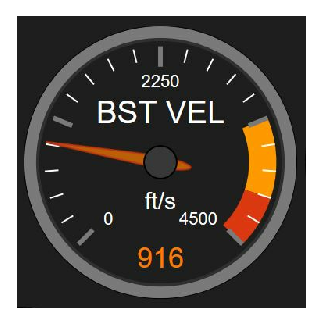
\includegraphics[width=120pt]{gauge.eps}}
\caption{Example Gauge}
\end{figure}
	\subsection{Acceleration}

		\subsubsection{GUI Element}
			The acceleration readout is actual composed of a gauge that will display the current acceleration being experienced by the rocket.
			
		\subsubsection{Structural Element}
			The acceleration gauge will have three zones.
			On the left of the gauge will be a normal, uncolored zone indicating an acceptable degree of acceleration.
			Working from left to right, next will be a yellow warning zone.
			Finally, on the right there will be a red danger zone indicating a potentially hazardous degree of acceleration.
			As the rocket does carry accelerometers, displaying acceleration data should require relatively little processing.

		\subsubsection{Design Rationale}
			These gauges allows positive readings; negative accelerations thus display the absolute value. 
      Direction (i.e. up or down) can be determined using other display components.
      This decision was made following user studies with the other members of the rocket team.
      The color-coding is an important aspect intended to allow for rapid visual assessment of flight status.
			The inclusion of an acceleration display provides critical information, most notably either excessively horizontal flight path (i.e. the rocket has become disoriented) or an uncontrolled descent (likely due to a parachute failure).

  \subsection{Temperature}

		\subsubsection{GUI Element}
			The temperature display consists of a gauge-type display element.
					
		\subsubsection{Structural Element}
			On the left of the gauge will be a normal, uncolored zone indicating an acceptable temperature.
			Working from left to right, next will be a yellow warning zone.
			Finally, on the right there will be a red danger zone indicating a potentially hazardous temperature.
						
		\subsubsection{Design Rationale}
			This gauge allows positive readings; negative temperatures thus display zero with the needle and the negative value with the attached text display. 
			The color-coding is an important aspect intended to allow for rapid visual assessment of flight status.
			That being said, however, the rocket is somewhat unlikely to experience a temperature which would actually be harmful given that the acceptable tolerance exceeds well beyond even the high desert temperatures expected.
    
  \subsection{Velocity}

		\subsubsection{GUI Element}
			The velocity display consists of a pair of gauges: one for vertical velocity and one for horizontal velocity.
			
		\subsubsection{Structural Element}
			In the center of each gauge will be a green zone indicating an acceptable velocity; zero will be located exactly in the middle.
			Working from the inside out, next will be a yellow warning zone.
			Finally, on the periphery there will be a red danger zone indicating a potentially hazardous velocity.
			Velocity will have to be derived from other values including coordinates and acceleration due to the lack of speedometers on the rocket.
			
		\subsubsection{Design Rationale}
			These gauges allow both positive and negative readings, a reflection of the fact that the rocket can and will move in both positive and negative directions with six degrees of freedom.
			The color-coding is an important aspect intended to allow for rapid visual assessment of flight status, particularly during the recovery stage (as excessive velocity during recovery indicates a likely parachute failure).
      
\begin{figure}[H]
\centering
\fbox{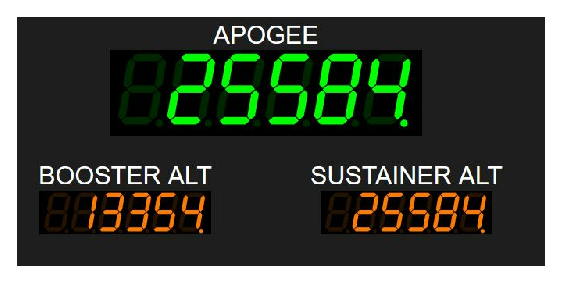
\includegraphics[width=240pt]{readouts.eps}}
\caption{Example Readouts}
\end{figure}      
      
	\subsection{Altitude}

		\subsubsection{GUI Element}
			The most logical way to display altitude is to use a numerical readout as this will allow users to quickly read the value (importantly this is a parameter where actual value is the most important aspect).
			The altitude readout should be prominent and easily visible on the display.
			Additionally, the client has expressed interest in the inclusion of audible cues indicating certain altitudes have been reached, should time allow (this is a flex goal).

		\subsubsection{Structural Element}
			As the rocket does carry barometric altimeters, displaying altitude data should require relatively little processing below 100,000 feet.
			After that point, commercially-available altimeters are no longer reliable, necessitating the derivation of altitude using other information.
			As the altitude readout is numerical, the most critical consideration is that it is properly sized to be easily readable.
			The inclusion of a color change upon reaching certain altitude thresholds can, however, make this even easier.
			
		\subsubsection{Design Rationale}
			As the overall goal of this project is to launch a student-built rocket to a minimum altitude, the display of altitude is critical to determining success.

  \subsection{GPS Coordinates}

		\subsubsection{GUI Element}
			The most logical way to display GPS Coordinates is to use a numerical readout, as this will allow users to quickly read the value (importantly this is a parameter where actual value is the most important aspect).
			The coordinate readout should be prominent and easily visible on the display.

		\subsubsection{Structural Element}
			As the rocket does GPS units, displaying coordinate data should require relatively little at certain speeds and altitudes.
			Above certain speeds and altitudes, commercially-available GPS units are no longer functional due to restrictions intended to prohibit their use in guided missiles, thus necessitating the derivation of coordinates using other information.
			As the coordinate readout is numerical, the most critical consideration is that it is properly sized to be easily readable.
			
		\subsubsection{Design Rationale}
      In addition to the actual flight component, another major consideration of this project is the timely recovery of both rocket stages post-flight.
      Displaying stage coordinates in numerical form will allow for a more precise location than simply using the 3D display discussed above, as the displayed coordinates can be read and subsequently entered into hand-held GPS units for use in the field.

      
\begin{figure}[H]
\centering
\fbox{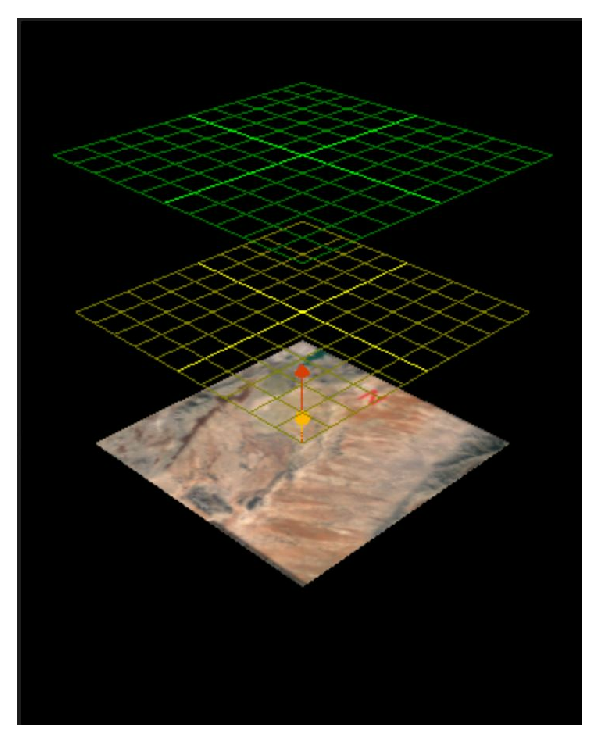
\includegraphics[width=120pt]{position.eps}}
\caption{Position Display}
\end{figure} 
	
	\subsection{Flight Path and Location}

		\subsubsection{GUI Element}
			The display of the rocket's flight path and location will actually be composed of two disparate elements.
			The most prominent of these will be a 3-dimensional representation of the launch area and target altitude planes, onto which will be projected representations of both rocket stages and their respective trajectories.
			The ground plane will use an image of the launch area as a texture, whereas the target planes will use a colored grid system.
			The target altitude of 150,000 feet will be green and the previous OSU record of 80,000 feet will be yellow.
			The second display element will take the form of a simple text readout of each stage's current GPS coordinates.
			Also worth noting is the fact that the 3-dimensional component of the display will allow the user to manipulate the eye position as needed.
			
		\subsubsection{Structural Element}
			Each rocket stage will carry a commercial GPS unit on-board, so for at least part of the flight the display of this information will be relatively straight-forward.
			Above certain altitudes and velocities, however, commercial GPS units are designed to shut off, a measure intended to prevent use on foreign ballistic missiles or rocket munitions.
			This means that for a portion of the flight, the location will need to be derived using other available data.
			For the trajectory history, a Bezier derivation or similar method will be used to produce a smooth curve given the reported position points.
			An important consideration for the 3-dimensional display is that the traditional x-y-z representation of GPS coordinates (where the ground is the x-y plane) differs from the representation in WebGL (where the ground is the x-z plane).
			This will necessitate a value swap at some point.

		\subsubsection{Design Rationale}
			The purpose of the flight path and location display is two-fold.
			Firstly, it serves as a tracking system while the rocket is in flight, and during this phase is a supplementary means of verifying rocket altitude.
			This informs the choice to include target altitude planes on the 3-dimensional display.
			The ability of the user to manipulate the eye position of the 3-dimensional display is included in recognition of the fact that the rocket could potentially move in such a way that a strictly-static view would inhibit effective observation.
			Secondly, this display is crucial during the recovery stage following flight.
			The inclusion of both simple GPS coordinates and a projection of location onto a map are both intended to facilitate the rapid location and recovery of both rocket stages.

	%\subsection{Data Storage}
	%
	%	\subsubsection{GUI Element}
	%		The data storage function will not be reflected on the main display page, as it should be occurring in the background and takes place entirely on the ground station itself.
	%		That being said, there should be a logging function on the base station which can be accessed from that hardware if needed.
	%
	%	\subsubsection{Structural Element}
	%		In accordance with the modular design of the system, the storage of data should be isolated from the display components.
	%		As both storage and display components will be working with the same information, they can both be passed duplicates of the processed telemetry, allow both components to operate simultaneously.
	%		In order to achieve a maximum degree of readability for future teams, the JSON data format (with paired name-value data) has been chosen for data storage.
	%
	%	\subsubsection{Design Rationale}
	%		Whereas the above functions serve an immediate purpose during and immediately proceeding the rocket's flight, the storage of data is intended for later review, either by future HART members or in the event of a catastrophic failure.
	%		As the above functions will be displaying all of the information which would be stored, the further inclusion of a display element to the storage function would be entirely redundant and serve only to distract users.
	%		As discussed earlier, however, the one exception to this would be the verbose logging of data storage on the ground station itself, if only as a means to ensure expected functionality.
	
\newpage

%-----------------------------------------------------------

\section{User Interface Design}


	\subsection{Overview}
		The overall goal of the Avionics Ground System User Interface is to make monitoring rocket status as simple as possible.
		To that effect, all a user should need to do to access the system is connect to the ground station's wireless router and navigate to a specified URL.
		All of the above-discussed information should then be displayed on a single page so that users can easily evaluate any and all telemetry data with a single glance and without the need for scrolling or other navigation.
		User interaction will in fact be kept to a relative minimum: with the exception of the 3-dimensional location and trajectory display, the user should have no need to interact with any of the display elements beyond simple observation.
	
	\subsection{Images}
    \begin{figure}[H]
    \centering
    \fbox{\includegraphics[width=480pt]{complete_dash.eps}}
    \caption{The HART Dashboard}
    \end{figure} 

	\subsection{Screen Object and Actions}
    In the above image, there are two main components: the 2D data "dashboard" on the left and the 3D position display on the far right.
    The 2D component includes an array of gauges and digital-style readouts intended to display relevant info about the rocket, including altitude, coordinates, acceleration, velocity, and temperature.
    The apogee display will also stop at the highest altitude achieved so that information will remain easily accessible post-flight.
		Beyond simply reading data, the primary means by which the user is able to interact is via the 3D position display.
    This portion of the dashboard allows for 3D rotation as well as zooming in and out.
    Importantly, this interactive functionality works both with mouse and touch input (on touch capable devices).
    This latter aspect was an important consideration given that the dashboard is intended to be used with both phones and laptops.
   
		
\end{document}